% author: Matheus Figueiredo

\documentclass {article}

\usepackage {tikz}
\usetikzlibrary {automata, positioning, arrows}

\begin{document}
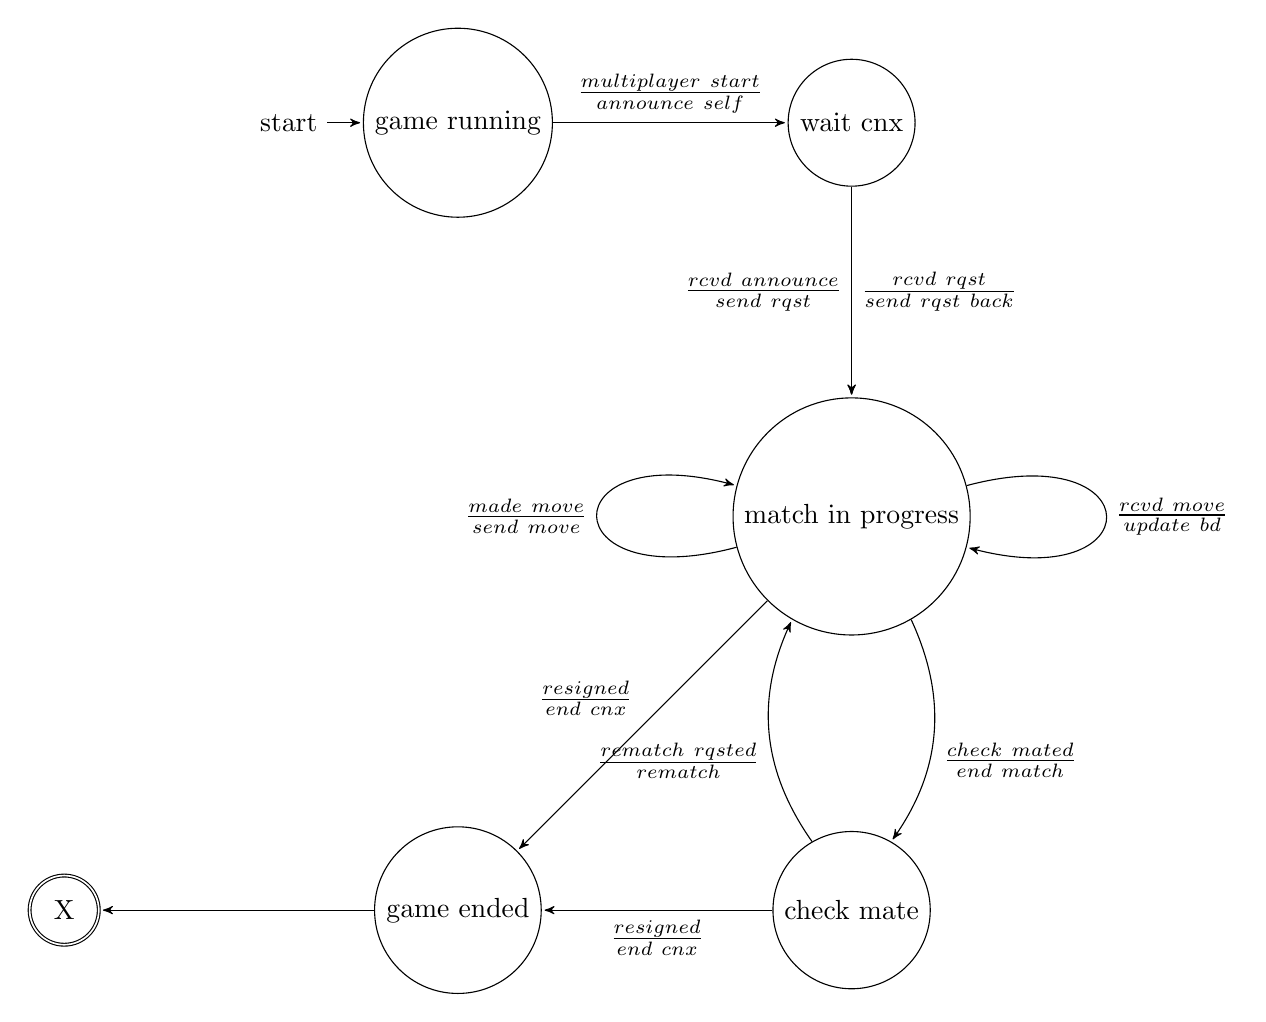
\begin{tikzpicture}[shorten >=1pt,node distance=5cm,on grid,auto]
  \tikzset{->, >=stealth'}
  
  \node[state,initial]  (q_0)                  {game running}; 
  \node[state]          (q_1) [right = of q_0] {wait cnx};
  \node[state]          (q_2) [below = of q_1] {match in progress};
  \node[state]          (q_3) [below = of q_2] {check mate};
  \node[state]          (q_4) [left  = of q_3] {game ended};
  \node[state,accepting](q_5) [left  = of q_4] {X};
  \path[->]
    (q_0) edge node {$\frac{multiplayer\ start}{announce\ self}$}   (q_1)
    (q_1) edge node {$\frac{rcvd\ rqst}{send\ rqst\ back}$}         (q_2)
          edge node [swap] {$\frac{rcvd\ announce}{send\ rqst}$}    (q_2)
    (q_2) edge [loop right] node {$\frac{rcvd\ move}{update\ bd}$}  (q_2)
          edge [loop left]  node {$\frac{made\ move}{send\ move}$}  (q_2)
          edge [bend left]  node {$\frac{check\ mated}{end\ match}$}(q_3)
          edge [swap]       node {$\frac{resigned}{end\ cnx}$}      (q_4)
    (q_3) edge [bend left] node {$\frac{rematch\ rqsted}{rematch}$} (q_2)
          edge node {$\frac{resigned}{end\ cnx}$}                   (q_4)
    (q_4) edge node {}                                              (q_5)
          ;
\end{tikzpicture}
\end{document}  
